\documentclass[reqno]{article}
\usepackage[utf8]{inputenc}

\title{Arie}
\author{luca}
\date{January 2020}

\usepackage{amssymb}
\usepackage{amsfonts}
\usepackage{amsmath}
%\usepackage[leqno]{amsmath}
\usepackage{scalefnt}
\usepackage{fancybox}
\usepackage{float}
\usepackage{natbib}
\usepackage{theorem}
\usepackage{lscape}
\usepackage{hyperref}
\usepackage{graphicx}
\usepackage{appendix}

\bibliographystyle{unsrtnat}

%\graphicspath{ {C:/Users/arieb/Dropbox/ambiguity/images/}}

\setcounter{MaxMatrixCols}{10}

\newtheorem{theorem}{Theorem}
\newtheorem{acknowledgement}[theorem]{Acknowledgement}
\newtheorem{algorithm}{Algorithm}
\newtheorem{axiom}[theorem]{Axiom}
\newtheorem{case}[theorem]{Case}
\newtheorem{claim}{Claim}[section]
\newtheorem{conclusion}[theorem]{Conclusion}
\newtheorem{condition}{Condition}
\newtheorem{conjecture}[theorem]{Conjecture}
\newtheorem{corollary}[theorem]{Corollary}
\newtheorem{criterion}{Criterion}
\newtheorem{definition}{Definition}
\newtheorem{example}{Example}
\newtheorem{exercise}[theorem]{Exercise}
\newtheorem{lemma}{Lemma}
\newtheorem{notation}[theorem]{Notation}
\newtheorem{problem}[theorem]{Problem}
\newtheorem{proposition}[theorem]{Proposition}
{\theorembodyfont{\upshape} 
\newtheorem{remark}{Remark}
}
\newtheorem{solution}[theorem]{Solution}
\newtheorem{summary}[theorem]{Summary}
\newenvironment{proof}[1][Proof]{\textbf{#1.} }{\ \rule{0.5em}{0.5em}}
\setlength{\evensidemargin}{1in} 
\setlength{\oddsidemargin}{1in} 
\setlength{\topmargin}{0.8in} 
\setlength{\voffset}{-0.85in} 
\setlength{\hoffset}{-0.9in} 
\setlength{\textwidth}{6.8in} 
\setlength{\textheight}{8.95in}   
\newtheorem{Assumption}{Assumption}
\newtheorem{Result}[theorem]{Result}
\renewcommand{\cite}{\citet}

\begin{document}

\title{Identification of Incomplete Preferences}
\author{Arie Beresteanu\thanks{%
Department of Economics, University of Pittsburgh, arie@pitt.edu. } \and %
Luca Rigotti\thanks{%
Department of Economics, University of Pittsburgh, luca@pitt.edu.}}
\date{January, 2020\thanks{%
We thank Richard Van Weelden for pointers and encouragements. We thank
Miriam Blumenthal for excellent RA work.}}
\maketitle

\begin{abstract}
This paper brings together two strands of recent literature: the one focused
on the consequences of incomplete preferences for economic outcomes, and the
one focused on the econometric identification of economic models that have
non-unique predictions. This connection is very natural because incomplete
preferences models typically yield multiplicity of outcomes. In particular,
we introduce an environment in which one can test the commonly held
assumption that preferences satisfy the completeness axiom using data
generated by the choices of heterogeneous individuals. We use methods from
random set theory, and results from the literature on partial
identification, to illustrate the connection between data and the
distribution of utility values in the population.

\bigskip

\noindent \textbf{Keywords}: Ambiguity, Incomplete Preferences, Knightian
Uncertainty, Partial Identification, Random Sets.

\bigskip

\textbf{Incomplete. Do not Cite. Do not distribute}.
\end{abstract}

\thispagestyle{empty}

\setlength{\baselineskip}{.26in}\newpage

\setcounter{page}{1}

%%%%%%%%%%%%%%%%%%%%%%%%%%%%
%%%     Introduction     %%%
%%%%%%%%%%%%%%%%%%%%%%%%%%%%

\section{Introduction}
\label{introduction}

This paper brings together two strands of recent literature: the one focused
on the consequences of incomplete preferences for economic outcomes, and the
one focused on the econometric identification of economic models that have
non-unique predictions.\footnote{Incompleteness in decision making under risk and uncertainty was first studied by \cite{Aumann62} and \cite{Bewley86} (eventually published as \cite{Bewley02}), and extended by \cite{DubraMaccheroniOk04}, \cite{Ok02}. Some applications of this work include \cite{RigottiShannon05}, and \cite{LopomoRigottiShannon11}.} This connection is very natural because
incomplete preferences models typically yield multiplicity of outcomes. In
particular, we introduce an environment in which one can test the commonly
held assumption that preferences satisfy the completeness axiom using data
generated by the choices of heterogeneous individuals. One says preferences
are complete when the decision maker can compare and rank any two
alternatives at her disposal. Without completeness, decision makers may not
be able to rank some alternatives. When this happens, behavior is
indeterminate in the sense that any choice among these alternatives is
possible. This indeterminacy is robust because incompleteness, unlike
indifference, is not easy to avoid. This is because indifference between two
alternatives is a knife-edge situation; it can be easily broken in the
direction of either one. Incompleteness, however, is not as easy to avoid.
Think, for example, of the incompleteness described by \textquotedblleft
thick indifference curves\textquotedblright ; in that case, small changes to
either alternative may not matter at all. For these reasons, indifference
differs in a fundamental way from incompleteness, and one cannot disregard
individuals who cannot compare alternatives. In bringing standard models to
data, one typically argues that an individual who is indifferent among two
alternatives is an extremely rare event because indifference is a knife-edge
situation. Therefore, this possibility can be ruled out based on zero
measure arguments. Without completeness, however, this reasoning no longer
holds and we cannot disregard the possibility that many individuals are
unable to rank the alternatives in front of them.

When using data to learn about the distribution of preferences in an
heterogeneous population, allowing for incompleteness poses what may seem
like an insurmountable problem. Since the theory says nothing about how
choices are made between incomparable alternatives, data cannot distinguish
between choices made because of a definite preference from choices made
randomly because two alternatives are incomparable. While in standard
discrete choice models this source of randomness is ruled out by the
assumption that everyone's preferences are complete, one may suspect that
when completeness is not imposed data cannot say anything about preferences.
To the contrary, we show that data can be used to learn about the
distribution of preference parameters without assuming the preferences of
all individuals are complete. The main difference is that instead of the
usual point identification, one can only obtain partial identification of
these parameters. We also show that, interestingly and surprisingly, under
some conditions one may be able to rule out the hypothesis that all
individuals in the population have complete preferences. These conditions
are given by the existence of observables that are correlated with choices
but orthogonal to preferences. When these instrumental variables exist,
completeness is a testable assumption.

In this paper we consider the simplest possible setting in which
incompleteness can have observable consequences when looking at data
collected by observing heterogeneous agents: a discrete choice model with
two alternatives. In the standard model with complete preferences, each
alternative is associated with a utility value which is known to the
decision maker but not known to the analyst. One then uses observed choices
to make inferences about the distribution of utility values in the
population. This inference is driven by the assumption that choices are made
in a utility maximizing fashion. Observing the proportion of individuals who
choose one alternative over another tells us that the same proportion must
assign higher utility to the corresponding alternative. In our initial
model, we weaken this framework by allowing for the possibility that each
alternative is associated with an interval of utility values. This
corresponds to the \emph{interval order} of \cite{Fishburn1970book}, who
calls the width of the interval associated to each alternative its \emph{%
vagueness}. When the intervals are disjoint, the alternatives can be ranked
and choice follows from utility maximization; when the intervals overlap,
the corresponding alternatives are not comparable and choice is
indeterminate.

We use methods from random set theory, and results from the literature on
partial identification, to illustrate the connection between data and the
distribution of utility values in the population. The observed proportion of
individuals who choose one alternative implies bounds on the probability
that any individual assigns a \textquotedblleft higher\textquotedblright\ or
\textquotedblleft lower\textquotedblright\ interval to that alternative.
Intuitively, these bounds follow from the observation that the fraction of
individuals who chooses one alternative gives an upper bound to the fraction
of individuals who assigns a higher interval to it. On the other hand, the
data cannot impose a lower bound to this same fraction as it could be the
case that all those who make one choice do it because they cannot compare it
to the other possibility. Based on these results, we conclude that discrete
choice data is informative about preference parameters even when
incompleteness is allowed.

The bounds described above are, by their very nature, compatible with the
possibility that all decision makers have complete preferences. As a matter
of fact, one cannot rule out the possibility that everyone in the population
has complete preferences. Intuitively, that is because individuals choose an
alternative for two possible reasons that the data cannot disentangle:
either that alternative has higher utility or it is not comparable to the
other possible choices. As a natural response to this situation, we focus on
finding conditions under which the data can actually rule out the
possibility that everyone's preferences are complete. In particular, we show
that an instrumental variable approach can yield these conditions. If there
is an observable variable that is orthogonal to preference parameters but
correlated with choice, it can be used to rule out the possibility that all
individuals have complete preferences.

Finally, we move to the most widely used model of incomplete preferences,
the Knightian Decision Theory of \cite{Bewley86}. In the framework of
decision making under uncertainty, that model derives a preference
representation where alternatives are compared in an expected utility
fashion, but using multiple probability distributions. One alternative is
preferred to another if it has higher expected utility for all probability
distributions in a closed convex set. In this model, comparisons are done
one probability distribution at a time; when all these comparisons agree,
the two alternatives can be ranked. Unlike the models so far, Bewley's
theory does not rank alternatives using an interval of utility values for
each. However, our previous results can be extended to this setting. Here,
the data provides bounds on the probability that the highest and lowest
expected utility difference between the two alternatives is negative.

\textbf{Structure of the paper} Section \ref{Background} reviews the two main ingredient of this paper: the theory of incomplete preferences and random set theory. Section \ref{randomDecisionMakers} discusses random decision makers and define the identification set for parameters of preferences distributions. Section \ref{BinaryChoice} covers binary choice models and Section \ref{DiscreteChoice}  general discrete choice. Section 6 Extends these results and discuss additional assumptions that may lead to point identification in section \ref{Voting} we apply our findings to a data set on voting in Ohio. Section \ref{conclustions} concludes.

%%%%%%%%%%%%%%%%%%%%%%%%%%%%
%%%%%    Background    %%%%%
%%%%%%%%%%%%%%%%%%%%%%%%%%%%

\section{Background
\label{Background}}

This paper combines two literatures. The first is the literature on partial identification using random set theory. The second is the literature on incomplete preferences. In this section we introduce the terminology and the basic results of these literatures that we use throughout this paper.
%%%%%%%%%%%%%%%%%%%
%%% Random Sets %%%
%%%%%%%%%%%%%%%%%%%

\subsection{Random Sets}
\label{RandomSets}
Identification analysis in economics has greatly benefited from tools developed in Random Set Theory (RST).\footnote{\cite{Molchanov2005} presents a general exposition of RST, while we focus on real-valued random variables and sets. The reader is referred to Appendix A of  \cite{BMM2012} and to \cite{Molchanov2005} for a more in depth discussion of RST.} We use results developed in \cite{BMM2011} and \cite{BMM2012} to identify the quantities and parameters of interest. Specifically, we focus on two sets of tools for the identification analysis: the Aumann integral approach and the containment functional approach. \footnote{\cite{BMM2012} discuss the merits of both approaches and make recommendations as to where each approach may have an advantage. In this paper we use both approaches.} In section \ref{nonpar} we use the containment functional whereas in section \ref{par} the Aumann integral approach is easier to apply. We start with defining random sets and then the concepts related to the two identification strategies that are used in later sections of this paper. 

\begin{Assumption}[probability space]\label{probSpace}
The probability space, $(I,\mathcal{F} ,P)$, on which all random variables and sets are defined is non-atomic.
\end{Assumption}

We use $i \in I$ to denote a random individual from the population $I$. From here on equalities and the statement "for every $i$" mean for every $i\in I$, $P$-a.s. 

\begin{definition}
A random set $X$ is a mapping $X:I \rightarrow \mathcal{K}\left(\mathbb{R}^{n}\right) $ where $\mathcal{K}\left(\mathbb{R}^{n}\right) $ is the set of all closed subsets of $\mathbb{R}^{n}$ and such that for all $K\subset \mathcal{K}\left(\mathbb{R}^{n}\right) $ compact, $\left\{ i:X\left( i\right) \cap K\neq \emptyset \right\} \in \mathcal{F}$.
\end{definition}

A random set can be thought of as a collection of point-valued random variables. For a random set $X$, we let $Sel\left(X\right)$ , the \textit{selection set} of $X$, be the collection of all (point-valued) random variables, $x$, defined on our probability space such that $x\left( i\right) \in X\left(i\right) $ for all $i$. Both identification approaches draw a relationship between a random set and its selections.

\subsubsection{Containment Functional Approach}
The containment functional of a random set corresponds to the distribution function of a random variable.

\begin{definition}
For a random set $X$ and $\forall K\in \mathcal{K}\left( \mathbb{R}^{n}\right) $, the containment functional is defined as%
\begin{equation*}
C_{X}\left( K\right) =P\left( X\subset K\right) .
\end{equation*}
\end{definition}

The following theorem ties between the selection and the containment functional. 

\begin{theorem}
(Artstein Inequalities) Let $X$ be a random set and let $Sel\left( X\right) $
be its selection set. Then $x\in Sel\left( X\right) $ if and only if 
\begin{equation*}
C_{X}\left( K\right) \leq P_{x}\left( K\right)
\end{equation*}%
for all $K\in \mathcal{K}\left( \mathbb{R}^{n}\right) $ where $P_{x}$ is the probability distribution of the random variable $x$.
\end{theorem}

When a single selection $x$ from the random set $X$ is observed, $P_x(K)$ is identified from the data. It can then be used to draw restrictions on the values that the containment functional can take. This approach is especially useful in case we look at projections of the random set and its selections on a lower dimensional space. We use this approach in section \ref{nonpar}.

\subsubsection{Aumann Expectation Approach}
 The selection set leads to a natural definition of expectation of random sets.

\begin{definition}
Let $X$ be a random set defined on a non-atomic probability space. If there is $x \in Sel(X)$ such that $E(x)$ is finite, then we say that the random set is integrable. The set of integrable selections of $X$ is denoted as $Sel^1(X)$. The Aumann expectation of an integrable random set $X$ is defined as 
\begin{align*}
    \mathbb{E}(X)=\{ E(x) : x \in Sel^1(X) \}\
\end{align*}
\end{definition}

The Aumman expectation of a random set produces a convex set (see \cite{Molchanov2005} Theorem 2.1.15). Convex sets can be characterize by their support function.

\begin{definition}
Let $A \subset \mathbb{R}^n$ be a convex set and let $\mathcal{B}$ be the unit sphere in $\mathbb{R}^n$. The support function $h: \mathcal{B} \rightarrow \mathbb{R}$ is defined as $h(u;A)=\sup_{a \in A} <u,a>$ for all $u \in \mathcal{B}$.
\end{definition}

The support function measures how far the set $A$ stretches in each direction. For a selection $x$ of $X$ we know its expectation must lie within the Aumann expectation of the random set. Since the last is a convex set, we can verify the inclusion of $E(x)$ in $\mathbb{E}(X)$ using the support function. This approach is useful when the random set is characterized by a finite parameter. We use this approach in section \ref{par}.

%%%%%%%%%%%%%%%%%%%%%%%%%
%%%     Vagueness     %%%
%%%%%%%%%%%%%%%%%%%%%%%%%

\subsection{Incomplete Preferences and Vagueness}
\label{Vagueness}
Our objective is to analyze the standard discrete choice model without
imposing the assumption that preferences are complete. In the standard
model, completeness is reflected by the idea that choice between alternative is driven by
the utility value assigned to each. This follows from the well
known result stating that, with a fine number of alternatives, for any complete and transitive
preference relation there exist a utility function representing those preferences. This utility function assigns a value to each alternative, and these values can be used to
describe choices made by a consumer who has those preferences. In other words, each alternative is associated with one number, and these numbers are used to model choices. Without completeness, this result no longer holds and one needs something that replaces it. For our purposes, any model in which each alternative is associated with two numbers, and these numbers determine choice behavior, will work. In what follows, we adopt a theory called interval orders (see \cite{Fishburn1970book}), but this is one of many possibilities.

We begin by presenting a model of decision making that allows preferences to be incomplete. Let $\mathcal{A}$ be universal set of alternatives.\footnote{%
In a more general setting each decision maker has a set $A(i)\subset \mathcal{A}
$ which is called the budget set and represents the alternatives feasible
for decision maker $i$. Although our analysis does not rule out different budget sets
for different agents, for simplicity we assume that all decision makers face the same set of alternatives.}

\begin{Assumption}[partial order]\label{alternatives} 
\label{intervalOrder} Let $\left( \mathcal{A},\succ \right)$ be a partially ordered set such that $\mathcal{A}$\ is a finite set and $\succ$ is a strict preference relation over $\mathcal{A}$ that satisfies the following two properties: (i) $\lnot \left( a\prec a\right) $ (where $\lnot $ denotes logical negation), and (ii) $a\prec b$ and $c\prec d$ 
$\Rightarrow $ $a\prec d$ or $c\prec b$.
\end{Assumption}

The first property is irreflexivity, while the second is a strong form of transitivity.\footnote{One can easily verify that (i) and (ii) immediately imply transitivity.} 
\cite{Fishburn1970book} calls such a preference an \textbf{interval order}, and it shows that $\succ$ can be represented using two functions as the following theorem illustrates.

\begin{theorem}[Fishburn (1970)] \label{Fishburn1970}
If $\succ $ is an interval order and $\mathcal{A}$ is finite, then there
exists two functions $\underbar{u}:\mathcal{A}\rightarrow \mathbb{R}$ and $\sigma :%
\mathcal{A}\rightarrow \mathbb{R}$ with $\sigma (a)>0$ for all $a\in A$,
such that%
\begin{equation*}
a\prec b\text{\qquad if and only if\qquad } \underbar{u} \left( a\right) +\sigma \left(
a\right) <\underbar{u}\left( b\right).
\end{equation*}
\end{theorem}

Thus, $b$ is preferred to $a$ if and only if the utility of $b$ exceeds the
utility of $a$ by some strictly positive amount. One can think of each
alternative as being associated with an interval on the real line. The lower
bound of that interval represents its utility, while the width of that
interval represents imprecision in that utility. In this spirit, Fishburn
calls $\sigma $ a \emph{vagueness} function since it measures the amount of
imprecision associated with each alternative. The name interval order
follows from the observation that alternatives are compared using intervals:
when $b$ is preferred to $a$ the interval $\left[ \underbar{u} \left( b\right) ,\underbar{u} \left( b\right) +\sigma \left( b\right) \right] $ lies to the right of the interval 
$\left[ \underbar{u} \left( a\right) ,\underbar{u} \left( a\right) +\sigma \left( a\right) \right] $. Interval orders are clearly not necessarily complete. When the two
intervals overlap, $a$ and $b$ are not comparable. In this setting, although
strict preference is transitive, incomparability is not. In other words, $a$
may be not comparable to $b$, and $b$ maybe not comparable to $c$, but $c$
is strictly preferred to $a$. This idea is sometimes referred to as
intransitive indifference.\footnote{Quoting from Fishburn: \textquotedblleft For example, if you prefer your coffee black it seems fair to assume that your preference will not increase as $x$, the number of grains of sugar in your coffee, increases. You might well be indifferent between $x=0$ and $x=1$, between $x=1$ and $x=2$, ... ,
but of course will prefer $x=0$ to $x=1000$.\textquotedblright}

In what follows, for ease of exposition, we let $\bar{u} (a)= \underbar{u} \left( a\right)
+\sigma \left( a\right) $ so that an alternative is associated with a pair
of numbers measuring the lower and upper bound of the alternative's `utility
interval'. Using these two values, one can then talk about behavior when
faced with a particular set of possibilities.

When only two alternatives are present, the choice implied by an interval
order is easy to describe. An alternative can be chosen if it is either
preferred to the other, or if it is not comparable to it. In other words, an
alternative can be chosen as long as it is not dominated. With more than two
alternatives, we extend this idea as follows: an alternative can be chosen
from a particular list of options provided there is no other option in the
list that is strictly preferred to it. We formalize this notion as follows.

\begin{definition}
The subset of $\mathcal{A}$ of \textbf{non-dominated alternatives} is defined as $$
M=\left\{ a\in \mathcal{A} :\forall b\in \mathcal{A},\ \bar{u}(a)\geq \underbar{u}(b)\right\}. $$
\end{definition}

The set $M$ is the set of all alternatives in $\mathcal{A}$ that
are not strictly dominated by another alternative. Without any further assumptions, the model may have multiple predictions. In other words, the model of discrete choice with interval utility is an incomplete model. We denote by $y$ the observable choice (selection) made by the decision maker and make the following assumption.

\begin{Assumption}[Rationality] \label{rationality}
Decision makers are rational and therefore, $y\in M$.
\end{Assumption}

With complete preferences, the set $M$ includes alternatives the
decision maker is indifferent among. Typical assumptions in empirical work ensure that $M$ is a singleton and thus $M$ and $y$ are synonymous. With interval order the set $M$ is not necessarily a singleton and may include several alternatives that the decision maker
cannot rank. This captures the idea that, although choice can be indeterminate, only the undominated alternatives can be chosen by the individual. In particular, this reflects the idea that no selection rule is a-priory imposed among incomparable alternative, provided none of them is strictly worse. On the other hand, an alternative that is strictly dominated is never chosen.\footnote{Using Fishburn's example, only cups of coffee which contains low amounts of sugar can be chosen. As soon as sugar content is high enough to make a cup of coffee with no sugar at all strictly better, that yields a dominated alternative. That cup, as well as any other that contains more sugar, will not be chosen.}


%%%%%%%%%%%%%%%%%%%%%%%%%%%%%%%%%%%%%
%%%     Random Decision Makers    %%%
%%%%%%%%%%%%%%%%%%%%%%%%%%%%%%%%%%%%%

\section{Random Decision Makers}
\label{randomDecisionMakers}

The notation set in section \ref{Background} refers to a single decision maker. We now turn to a situation where there are many decision makers with heterogeneous preferences. We maintain the assumption that the universal set of alternatives faced by all decision makers is $\mathcal{A}$ which satisfies
assumption \ref{intervalOrder}.

As in Section \ref{RandomSets}, let $(I,\mathcal{F} ,P)$ be a non-atomic probability space satisfying assumption (\ref{probSpace}). We use $i \in I$ to denote a random individual from the population $I$. Every decision maker $i\in I$ has an interval order over the set of choices $\mathcal{A}$ that satisfies Assumption \ref{alternatives}. By Theorem \ref{Fishburn1970} we can say that for each $a\in \mathcal{A}$, decision maker $i$ has a utility interval $\left[ \underbar{u} \left( a,i\right) ,\bar{u}\left( a,i\right) \right] $. We can, therefore, treat $\underbar{u}$ and $\bar{u}$ as two random functions defined on  $\mathcal{A}$ such that for every $a\in \mathcal{A}$, $\Pr \left[ \underbar{u}(a)\leq \bar{u}\left( a\right) \right] =1$. We are interested to learn about the joint distribution of utilities $\mathcal{U} = \{ \left(\underbar{u}\left( a\right) ,\bar{u}\left( a\right) \right) \}_{a \in \mathcal{A}}$ or features of this distribution using the joint distribution of the observed variables. We denote the joint distribution of $\mathcal{U}$ by $P_{\mathcal{U}}$.

For $i\in I$ we denote by $M(i)$ the set of alternatives that are not dominated.\footnote{The set $M(i)$ should be indexed by $\mathcal{U}$ to denote that it depends on the joint distribution of $\mathcal{U}$ which we want to identify. For simplicity we use $M(i)$ instead of $M_\mathcal{U}(i)$.} In other words, 

\begin{align}
\begin{split}
\label{choiceSet}
M(i) &=\{a \in \mathcal{A} : \nexists b \in \mathcal{A} \text{ such that } \underbar{u}(b,i)> \bar{u}(a,i) \} \\
&= \{a \in \mathcal{A} : \max\limits_{b \in \mathcal{A}} \underbar{u}(b,i) <  \bar{u}(a,i) \}.
\end{split}
\end{align}

Since $\mathcal{A}$ is a finite set, $M(i)$ is non-empty and therefore $M$ is a random set. 

%%%%%% nonparametric approach %%%%%%

\subsection{Nonparametric approach}\label{nonpar}
Let $\theta $ denote a certain parameter of the joint distribution of $\mathcal{U}$. For example, $\theta =\Pr\left( \bar{u}(b) \leq \underbar{u}(a) \right)$ which is the probability mass of decision makers for which alternative $a$ strictly dominates alternatives $b$. In this section we leave the distribution of $\mathcal{U}$ unspecified. Let $\Theta $ be the set of all feasible values that $\theta $ can take. $\Theta $ is called the parameter space. In our example, $\Theta=[0,1]$. In this section we show how can we use observational data to partially identify parameters of interest.

Consider the random set $M$ defined in equation (\ref{choiceSet}). The distribution of the random set $M$ can be represented by its containment functional $C_M$. The values that the random set $M$ takes and the value of its containment functional depend on the unknown joint distribution of $\mathcal{U}$. 

Assumption \ref{rationality}, rationality, implies that the choice of individual $i$, $y_i$ is an element of the set $M(i)$. In the context of random set theory, this behavioral assumption translates to the following measurability assumption.
\begin{Assumption}[measurability]
the random variable $y$ is a selection of the random set $M$.
\end{Assumption}
Therefore, rationality implies that the random variable $y$ is a selection from the random set $M$. 

For any $K\subset \mathcal{A}$, the choice probabilities $\Pr (y\in K)$ are identified from the data generating process. Following Artstein's Lemma, we can say that $y$ is a selection of $M$ if and only if for all $K\subset \mathcal{A}$, 
\begin{equation}
C_{M}(K)\leq \Pr (y\in K).  \label{containment_inequality}
\end{equation}
Computing the containment functional gives, 
\begin{align*}
C_{M}(K)& =\Pr (M\subset K) \\
& =\Pr (M\cap K^{c}=\varnothing ) \\
& =\Pr (\underset{k\in K^{c}}{\max }\bar{u}(k)<\underset{a\in \mathcal{A}}{\max }%
\text{\b{u}}(a)) \\
& =\Pr (\underset{k\in K^{c}}{\max }\bar{u}(k)<\underset{a\in K}{\max }%
\text{\b{u}}(a))\text{.}
\end{align*}

Inequality (\ref{containment_inequality}) imposes restrictions on the joint distribution of the random variables $\mathcal{U}$. Let $\mathcal{P}$ be the family of all probability distributions over the set $\mathcal{U}=\{\text{\b{u}}(a),\bar{u}(a)\}_{a\in \mathcal{A}}$ such that $\text{\b{u}}(a) \leq \bar{u}(a)$ for all $a\in \mathcal{A}$ with probability $1$. Given our knowledge of $\{\Pr(y\in K)\}_{K\subset \mathcal{A}}$, the identification region is defined as%

\begin{equation} \label{idRegion}
\mathcal{P}^{I}=\{P\in \mathcal{P} :C_{M}(K)\leq \Pr (y\in K) \; \forall K\subset \mathcal{A} \}\text{.}
\end{equation}

Artstein's Lemma implies that the set $\mathcal{P}^I$ is the sharp identification region for the set of joint distributions on $\mathcal{U}$. Appendix \ref{nonparAppendix} provides two results that shows how essential are the inequalities implied by Artstein's Lemma.

With no further restriction on the joint distribution of $\mathcal{U}$ beyond $\underbar{u}\left( a\right) \leq  \bar{u} \left( a\right)$, we cannot say anything further. There are two possible ways to make progress. First, the joint distribution of $\mathcal{U}$ can be assumed to belong to a finite parameter family and we can seek to partially identify this parameter. We take this approach in Section \ref{par}. Second, we can avoid parametric assumptions but limit our interest to a finite number of features of the joint distribution of $\mathcal{U}$. We proceed in this direction in Sections \ref{BinaryChoice} and \ref{DiscreteChoice}. 

%%%%%%% Parametric approach
\subsection{Parametric approach}\label{par}
Suppose first that the joint distribution of $\mathcal{U}$ is characterized by a finite dimensional parameter $\theta \in \Theta \subseteq  \mathbb{R}^k$. We denote this distribution as $P_{\theta}$. 

For $\theta \in \Theta$, let $\underbar{u}_{\theta}(a,i)$ and $\bar{u}_{\theta}(a,i)$ be the lower and upper utilities for decision maker $i$ for alternative $a \in \mathcal{A}$ given the parameter is $\theta$. For $i\in I$ we denote by $M_{\theta}(i)$ the set of alternatives that are not dominated. In other words, 

\begin{align}
\begin{split}
M_{\theta}(i) &=\{a \in \mathcal{A} : \nexists b \in \mathcal{A} \text{ such that } \underbar{u}_{\theta}(b,i)> \bar{u}_{\theta}(a,i) \} \\
&= \{a \in \mathcal{A} : \max\limits_{b \in \mathcal{A}} \underbar{u}_{\theta}(b,i) <  \bar{u}_{\theta}(a,i) \}.
\end{split}
\end{align}

The identification region in equation (\ref{idRegion}) can be written as
\begin{align}
    \Theta^{I} = \{ \theta \in \Theta : C_{M_{\theta}}(K)\leq P_{\theta}(y\in K) \text{ } \forall K\subset \mathcal{A} \}\text{.}
\end{align}

For each $m \in Sel(M)$, we define a random variable $q(m)$ who gets its values in $ \Delta^{| \mathcal{A} |}$ such that $[q(m(i))]_k=1[m(i)=k]_{k=1.. | \mathcal{A} |}$ and $1[\cdot]$ is the indicator function. In other words, $q(m)$ is a random vector whose entries all equal to zero except from the coordinate that represents the choice made by $i$. The expected value of this random vector $E(q(m))$ is a point in the simplex $\Delta^{| \mathcal{A} |}$ represents the distribution of choices.

We define the following random set 
\begin{equation}
    Q(M) = \{ q(m) : m \in Sel(M) \}.
\end{equation}
The random set $Q(M)$ represents all the possible choices that our incomplete model can predict. $Q(M)$ is a random set who takes its values in $\Delta^{| \mathcal{A} |}$. Hence, the Aumann integral of $Q(M)$ is well defined,

\begin{equation}
    \mathbb{E}(Q(M)) = \{E(q) : q \in Sel(M)\}.
\end{equation}

We say that the set $\mathbb{E}(Q(M))$ is the set of model predictions for choice distributions. This set includes all the distributions over the finite set $\mathcal{A}$ that may result from the distribution of incomplete preferences $\mathcal{U}$. 

Let $y_{i}$ denote the observed choice made by $i$, such that $y_{i}\in \mathcal{A}$. We may also observe additional vectors of relevant covariates for individual $i$ depending on the context. For simplicity we avoid conditioning on these variables in this section. The observed choice, $y$ is assumed to satisfy Assumption \ref{rationality}, rationality. In other words, we assume that $y \in Sel(M)$. Using Theorem 2.1 in BMM (2012), the identification region for $P_{\mathcal{U}}$ is, 

\begin{equation}
    \Theta^I = \{ P : \min_{v \in \mathcal{B}}(E[h(Q(M),u)] - u'P(y)) \}
\end{equation}
where $\mathcal{B}$ is the unit ball in $\mathbb{R}^{| \mathcal{A} | - 1}$ and $h(A,v)$ is the support function of a set $A \subset \mathbb{R}^{| \mathcal{A} | - 1}$ evaluated in direction $v \in \mathcal{B}$.
%%%%%%%%%%%%%%%%%%%%%%%%%%%%%
%%%     Binary Choice     %%%
%%%%%%%%%%%%%%%%%%%%%%%%%%%%%
\section{Binary Choice}
\label{BinaryChoice}

In this section we focus on a binary choice models. Let the set of alternatives be $\mathcal{A}=\left\{ a_0,a_1\right\} $ for all $i$. Let $u_{i}(a) = [\underbar{u}(a) , \bar{u} (a) ] $. This is the interval utility that agent $i$ assigns to alternative $a \in \mathcal{A}$. This model assumes that the interval is known to the decision maker and thus she can maximize her utility.

Let $y_{i}=\mathbf{1}\left[ u_i(a_1)>u_i(a_0)\right]$. We denote the choice probability of alternative $a_1$ by $p_1 = \Pr \left( y_{i}=a_1\right)$ and the choice probability of $a_0$ by $p_0=\Pr \left( y_{i}=a_0\right)$. It is clear that $p_{1}=\Pr \left( V>0\right) $ and $p_{0}=\Pr \left( V<0\right) $.%
\footnote{We assume that $V$ is a continuous variable and thus $\Pr \left( V=0\right)
=0$ and thus we can ignore this event or add it to any other event.}
Typically $y$ is observed while $V$ is known only to the agent but is unobserved by us. \ Therefore, the DGP identifies $p_{0}$ and $p_{1}$ and thus it identifies $\Pr \left( V<0\right) $ and $\Pr \left( V>0\right) $
respectively. In \ the literature on discrete choice it is common to specify a distribution function for $V$ which is known up to a finite parameter $\theta $. In this case, $\theta $ can be consistently and efficiently
estimated by maximum likelihood.

Suppose now that $V=[V_{L},V_{U}]$ where $V_{L}$ and $V_{U}$ are two random variables such that $\Pr \left( V_{L}\leq V_{U}\right) =1$. We fix $u\left(0\right) $ to be a singleton. In practice the decision maker can face
vagueness with respect to the utility from choice $0$ as well. Since what matters is the order of the utilities resulting from alternatives $0$ and $1$, we can think about $V$ as the Hukuhara difference (see \cite{Hukuhara1967}%
) between the random sets representing the utility from alternative $1$ and alternative $0$.

Given this vagueness about the utility from alternative $1$, the decision maker's choice set is
\begin{equation*}
Y=\left\{ \begin{array}{c}
\{1\} \\ 
\{0,1\} \\ 
\{0\}
\end{array}
\ 
\begin{array}{c}
\ V_{L}>0 \\ 
0\in \left[ V_{L},V_{U}\right] \\ 
V_{U}<0%
\end{array}%
\right. .
\end{equation*}%
When $0\in \left[ V_{L},V_{U}\right] $ the decision maker is unsure how to
rank the two options she faces. Figure \ref{fig:choicerule} illustrates the
decision rule.

\begin{figure}[h!]
    \centering
    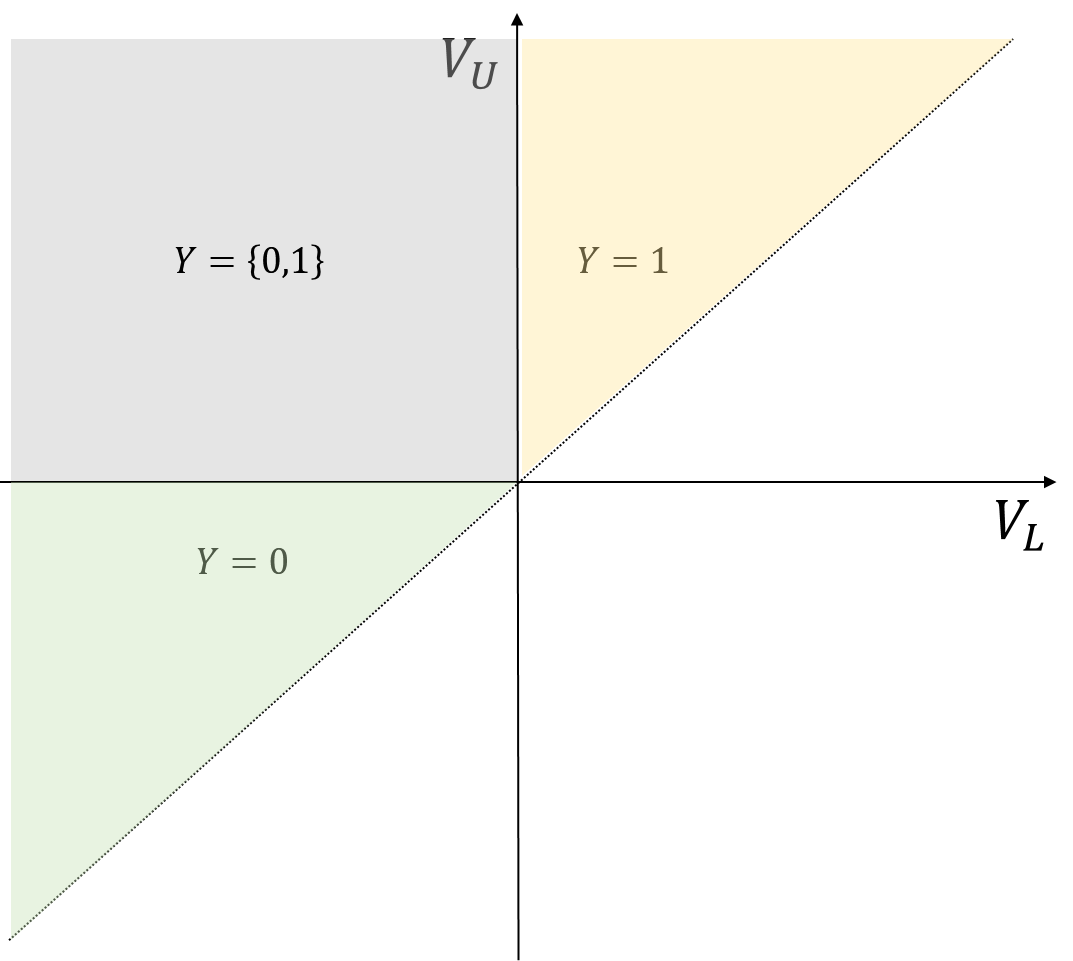
\includegraphics[scale=0.6]{choicerule}
    \caption{Choice Rule with Incomplete Preferences}
    \label{fig:choicerule}
\end{figure}

As above, we denote the agent's choice by $y$. Following Artstein inequality
\footnote{See \cite{Molchanov2005} Theorem 2.20 and Theorem 2.1 in \cite{BMM2012}.}
$y\in Sel\left( Y\right) $ if and only if $\Pr \left( y\in K\right) \geq
C_{Y}\left( K\right) $ for every closed set $K$ where $C_{Y}\left( K\right) $ is the containment functional defined as $C_{Y}\left( K\right) =\Pr \left( Y\subset K\right) $. Since $C_{Y}\left( \{0\}\right) =\Pr \left(
V_{U}<0\right) $ and $C_{Y}\left( \left\{ 1\right\} \right) =\Pr \left(
V_{L}>0\right) $, for any $y\in Sel\left( Y\right) $, $\Pr (y=0)\geq \Pr
\left( V_{U}<0\right) $ and $\Pr \left( y=1\right) \geq \Pr \left(
V_{L}>0\right) $. Using the fact that $\Pr \left( y=0\right) =1-\Pr (y=1)$,
we can conclude that
\begin{equation}
\Pr \left( V_{U}<0\right) \leq \Pr (y=0)\leq \Pr \left( V_{L}<0\right) .
\label{Artstein}
\end{equation}%
Without observing $y$\ the probability $\Pr \left( y=0\right) $ is
unidentified and inequality (\ref{Artstein}) implies only that $\Pr \left(
V_{U}<0\right) \leq \Pr \left( V_{L}<0\right) $. This is immediate from our
initial assumption that $\Pr \left( V_{L}\leq V_{U}\right) =1$. Suppose we
observe data on choices made by decision makers facing the type of
incompleteness described above. Since we can identify $p_{1}$ and $p_{0}$
from the data, inequality (\ref{Artstein}) becomes%
\begin{equation}
\Pr \left( V_{U}<0\right) \leq p_{0}\leq \Pr \left( V_{L}<0\right) .
\label{ineq1}
\end{equation}%
Without further assumptions this is the only information we can draw about
the joint distribution of $V_{L}$ and $V_{U}$. We cannot reject, for
example, the hypothesis that $V_{L}=V_{U}$, $P-a.s.$ and there is no
vagueness about choice $1$. \ Moreover, the above inequality bound the
marginal cumulative distributions of $V_{L}$ and $V_{U}$ at the point $0$
but does not provide information on their joint distribution or other
features of their marginal distributions. Another parameter of interest here
is the proportion of decision makers who have incomplete preferences. This
proportion is $\Pr \left( V_{L}<0\ \wedge V_{U}>0\right) =1-\Pr \left(
V_{L}>0\right) -\Pr \left( V_{U}<0\right) =\Pr \left( V_{L}<0\right) -\Pr
\left( V_{U}<0\right) $. Again, this quantity can be anywhere between zero
and one.

\begin{figure}[h!]
    \centering
    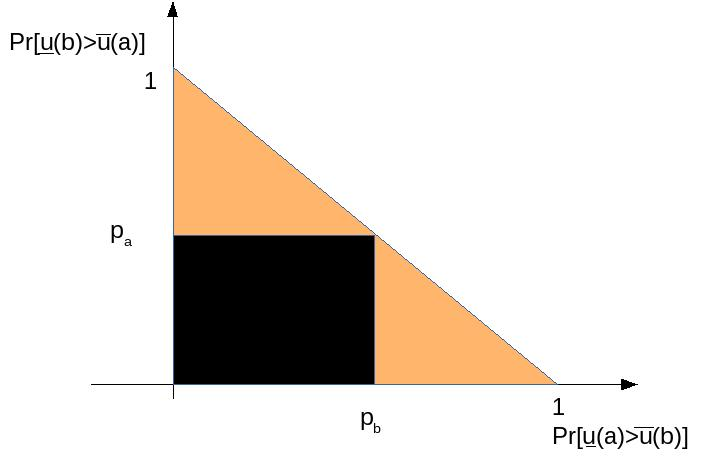
\includegraphics[scale=0.6]{idregion2.jpg}
    \caption{Partial identification with Two Alternatives}
    \label{fig:impreciseutilityidentification}
\end{figure}

Figure \ref{fig:impreciseutilityidentification} illustrates the information
contained in inequality (\ref{ineq1}). Before observing any data the only
information we have is that $V_{L}\leq V_{U}$ for every individual $i$.
Therefore, $\Pr \left( V_{L}<0\right) \geq \Pr \left( V_{U}<0\right) $. The
area under the $45{{}^\circ}$ line represents this information. After observing data we can identify the
frequency $p_{0}=\Pr \left( y=0\right) $. Inequality (\ref{ineq1}) then puts
restrictions on the values that the cumulative distributions of $V_{L}$ and $%
V_{U}$ can take at the point $0$. For example, say $p_{0}=0.37$. We can no
longer admit the case where $\Pr \left( V_{L}<0\right) =0.3$ and $\Pr \left(
V_{U}<0\right) =0.25$. Similarly we cannot admit the case where $\Pr \left(
V_{L}<0\right) =0.5$ and $\Pr \left( V_{U}<0\right) =0.4$. The two triangles
corresponding to these cases are eliminated from the identification region
after observing data. The remaining identification region is the rectangle
north-west of the point $\left( p_{0},p_{0}\right) $. Note that the case
where $\Pr (V_{L}<0)=\Pr \left( V_{U}<0\right) =0.37$ is included in the
identification region. The fact that these two probabilities are equal to
each other does not necessarily mean that there is no incompleteness and
that $V_{L}=V_{U}$ for all $i$. It is still possible that the quality of
choice $1$ is not known to the agent precisely but $\Pr \left(
0<V_{L}<V_{U}\right) =0.37$ and $\Pr \left( V_{L}<V_{U}<0\right) =0.63$. In
other words, there is incompleteness but it is choice irrelevant.

The point $\left( p_{0},p_{0}\right) $ in Figure \ref%
{fig:impreciseutilityidentification} represents a situation where $\Pr \left(
V_{U}<0\right) =p_{0}=\Pr \left( V_{L}<0\right) $ and therefore no DM has
incomplete preferences. On the otherhand the point $\left( 1,0\right) $
represents a situation where $0=\Pr \left( V_{U}<0\right) <\Pr \left(
V_{L}<0\right) =1$ and all DMs cannot rank the two alternatives. It is
natural to ask what is the identification region if we know that at least a
proportion $\alpha \in \left( 0,1\right) $ of decision makers cannot rank
the alternatives. Using the same reasoning as above, we have $\alpha \leq
\Pr \left( V_{L}<0\ \wedge V_{U}>0\right) =1-\Pr \left( V_{L}>0\right) -\Pr
\left( V_{U}<0\right) =\Pr \left( V_{L}<0\right) -\Pr \left( V_{U}<0\right) $%
. Therefore, this information adds the restriction that 
\begin{equation}
\Pr \left( V_{U}<0\right) \leq \Pr \left( V_{L}<0\right) -\alpha .
\label{ineq2}
\end{equation}


Figure \ref{impreciseutilityidentification2} depicts the identification
region consistent with both inequalities (\ref{ineq1}) and (\ref{ineq2}).
The dark region in Figure \ref{impreciseutilityidentification2} includes all
the points which are consistent with the statement that at least an $\alpha $
proportion of the DMs cannot rank the two alternatives in addition to the
observation that $p_{0}$ portion of DMs eventually chose alternative $0$.

The theory we have presented so far makes few assumptions. Our results
illustrate that identification, albeit partial, is possible when preferences
are not complete. Next, we illustrate how further assumptions can lead to
even stronger conclusions in terms of identification. First, we briefly
discuss assumptions on the joint distribution of $\left( V_{L},V_{U}\right) $%
. Then, we show that the presence of particular instruments can lead to a
rejection of the hypothesis that all consumers' preferences are complete.
Finally, we discuss a possible way to break incompleteness using the idea of
regret.

\begin{example}
Let $A=\{0,1\}$. Let $\text{\b{u}}(0)=\bar{u}(0)=0$. Let $\text{\b{u}}(1)=\beta -\varepsilon$ where $\varepsilon \sim F_{\varepsilon }$ such that $F_{\varepsilon }$ is known and $E[\varepsilon ]=0$. Let $\bar{u}(1)=\text{\b{u}}(1)+\sigma $ where $\sigma \in \mathbb{R}_{+}$. Let $y\in A$ be the choice made under rationality. We observe $p_{0}=\Pr (y=0)$ and $p_{1}=\Pr (y=1)$. Let $H$ be the set of all pairs $
(\beta ,\sigma )$ that are consistent with the observed $(p_{0},p_{1})$. 
\newline
\relax\textbf{Case 1} (no vagueness): Assume $\sigma =0$. $p_{1}=\Pr
(y=1)=\Pr $ $(\beta -\varepsilon >0)=\Pr (\varepsilon <\beta
)=F_{\varepsilon }(\beta )$. Therefore, $\beta =F_{\varepsilon }^{-1}(p_{1})$%
. The identification set is a singleton 
\begin{equation*}
H=\{(F_{\varepsilon }^{-1}(p_{1}),0)\}\text{.}
\end{equation*}%
\newline
\relax\textbf{Case 2} (vagueness): $\sigma \in \mathbb{R}_{+}$. We know that $p_{1}\geq \Pr (\text{\b{u}}(1)>0)=\Pr (\beta -\varepsilon
>0)=\Pr (\varepsilon <\beta )$. We also know that $p_{0}\geq \Pr
(\bar{u}(1)<0)=\Pr (\beta +\sigma -\varepsilon <0)=\Pr (\varepsilon >\beta
+\sigma )=1-F_{\varepsilon }(\beta +\sigma )$. These inequalities imply that 
$F_{\varepsilon }(\beta )\leq p_{1}\leq 1-F_{\varepsilon }(\beta +\sigma )$.
In other words, $\beta \leq F_{\varepsilon }^{-1}(p_{1})\leq \beta +\sigma $%
. The identification set is 
\begin{equation*}
H=\{(\beta ,\sigma )\in \mathbb{R} \times \mathbb{R}_{+}:\beta <F_{\varepsilon }^{-1}(p_{1})<\beta +\sigma \}\text{.}
\end{equation*}%
This identification region contains the point $(F_{\varepsilon
}^{-1}(p_{1}),0)$. \newline
\relax\textbf{Case 3} (instrumental variable): As in Case 2, $\sigma \in \mathbb{R}_{+}$ but now we observe a random variable $Z$ with support $Z$ such that $Z$
does not affect the valuation but it may affect the choice in case of
incompleteness. In other words, $\beta $ is not a function of $Z$ and $%
\varepsilon $ is independent of $Z$. We observe $p_{0|z}=\Pr (y=0|Z=z)$ and $%
p_{1|z}=\Pr (y=1|Z=z)$ for all $z\in Z$. Following the same analysis as
above we can conclude that $\beta \leq \underset{z\in Z}{\min }%
F_{\varepsilon }(p_{1|z})$ and $\underset{z\in Z}{\max }F_{\varepsilon
}^{-1}(p_{1|z})\leq \beta +\sigma $. The identification set is%
\begin{equation*}
H=\{((\beta ,\sigma )\in \mathbb{R} \times \mathbb{R}_{+}: \beta \leq \underset{z\in Z}{\min }F_{\varepsilon }(p_{1|z}),\underset{%
z\in Z}{\max }F_{\varepsilon }^{-1}(p_{1|z})\leq \beta +\sigma )\}\text{.}
\end{equation*}

We can immediately see that if $\underset{z\in Z}{\max }F_{\varepsilon
}^{-1}(p_{1|z})>\underset{z\in Z}{\min }F_{\varepsilon }(p_{1|z})$, we can
rule out all points for which $\sigma =0$. In other words, if for different
values of $Z$ there are different choice probabilities this can only be a
result of ambiguity. \newline
\relax
\end{example}

\begin{example}
Let $A=\{a_{0},a_{1},a_{2}\}$ be the alternatives set. Suppose we normalize $%
\text{\b{u}}(a_{0})=\bar{u}(a_{0})=0$. This is not a trivial normalization but we
make this assumption for two reasons. First, we need a location and scale
normalizations. This can be achieved by fixing the utility of alternative $%
a_{0}$ to zero and by setting the error terms distribution to one that has a
fixed variance. Second, to have a tractable example, we want to reduce the
number of parameters to be evaluated. For the other alternatives in $A$ we
assume%
\begin{equation*}
\text{\b{u}}(a_{j})=\beta _{0}+\beta _{1}X_{j}-\varepsilon
_{j},\bar{u}(a_{j})=\text{\b{u}}(a_{j})+\delta _{j}\text{,}
\end{equation*}%
where $j=1,2.$ The parameter to be evaluated is $\theta =\{\beta _{0},\beta
_{1},\delta _{1},\delta _{2}\}\in \mathbb{R}^{2} \times \mathbb{R}_{+}^{2}$. For simplicity we assumed that the intercept and slope in $V_{L}$
are the same for both alternatives $a_{1}$ and $a_{2}$. To make this example
tractable we assume that $\varepsilon _{1}$ and $\varepsilon _{2}$ are
independent of each other and independent of the covariate $X$. If we assume
that $(\varepsilon _{1},\varepsilon _{2})$ are jointly Normal with vector
mean $0$ and the identity variance-covariance matrix $I_{2\times 2}$, we
have a Probit model with quality ambiguity. A similar extension of the Logit
model can be made if we assume a T1EV distribution instead. Denote the
cumulative distribution of $\varepsilon _{j}$ as $\Phi $ for both $j=1,2$.
To simplify notation, we are omitting conditioning on $(X_{1},X_{2})$ in all
probabilities below. Similarly to the discussion above we can see that 
\begin{align*}
1-\Pr (\bar{u}(a_{j})& \geq \underset{k\in \{j\}^{c}}{\max }\text{\b{u}}(a_{k})) \\
& \geq p_{j}=\Pr (y=j) \\
& \geq \Pr (\text{\b{u}}(a_{j})\geq \underset{k\in \{j\}^{c}}{\max }\bar{u}(a_{k}))%
\text{.}
\end{align*}%
Applying our assumptions we get 
\begin{align*}
& \Phi (\beta _{0}+\beta _{1}X_{1}+\delta _{1})\cdot \Phi (\beta _{0}+\beta
_{1}X_{2}+\delta _{2}) \\
& \leq p_{0}\leq \\
& 1-[1-\Phi (\beta _{0}+\beta _{1}X_{1})]\cdot \lbrack \Phi (\beta
_{0}+\beta _{1}X_{2})]
\end{align*}%
and similarly we can find inequalities for the other probabilities.
\end{example}

\textbf{Numerical example}

Consider the following model. The alternatives set is $A=\left\{
a_{0},a_{1},a_{2}\right\} \text{.}$ We make the following normalizations.
For $i\in \left\{ 0,1,2\right\} \text{,}$ 
\begin{align}
\text{\b{u}}\left( i\right) & =\beta _{i}+\varepsilon _{i} \\
\bar{u}\left( i\right) & =V_{L}\left( i\right) +\sigma +\eta _{i}
\end{align}%
We set $\beta _{0}=0$ and $\sigma =1$. Therefore, we have only two
parameters to identify: $\beta _{1}$ and $\beta _{2}$. We made the following
parameter choice,%
\begin{equation}
\mathbf{\beta }=\left( 0,0.094,-0,054\right)
\end{equation}%
We let $\varepsilon _{i}$ and $\eta _{i}$ be i.i.d U$\left[ -0.25,0.25\right]
$. A data of $7250$ observations simulated from the above model was
generated. In other words, for each of the simulated $7250$ individuals we
generated $3$ intervals represented their utility intervals for the $3$
alternatives. We then had to make an arbitrary choice how these decision
makers break ambiguity. There are of course many ways to do that. Our choice
was to compute the mid-point of the $3$ intervals and to pick the
alternative with the highest value. As a result the sample we generated
produced the following choice probabilities vector for the $3$ alternatives,%
\begin{equation}
p=\left( 0.181,0.766,0.053\right) .
\end{equation}%
This vector is then passed to the next stage where we identify which pairs
of To check whether a certain pair of parameters is in the identification
region we have to verify $6$ inequalities. To do that we calculate the
capacity functionals by simulation and compare them to the vector of choice
probabilities above. The following scatter plot was generated using a
differential evolution algorithm.


\section{Discrete Choice with Incomplete Preferences}\label{DiscreteChoice}

Our leading model is discrete choice. Denote the set of alternatives that
each decision maker faces as $\mathcal{A}=\left\{
a_{0},a_{1},...,a_{J}\right\} $. Let $V:I\rightarrow \mathbb{R}^{\mathcal{A}}$ denote the (random) utility vector that each decision maker $i$ assigns to the alternatives in $\mathcal{A}$. For simplicity, we denote the vector of utilities for $i$ as $V_{i}=\left( V_{i0},V_{i1},...,V_{iJ}\right) $. We denote the choice of decision maker $i$ by $y_{i}=\arg \max_{j\in \mathcal{A}}V_{ij}$. We also denote the choice
probabilities by $p_{j}=\Pr \left( y_{i}=j\right) $. If all $V_{ij}$ are
single valued, this is the regular discrete choice model where $p_{j}=\Pr
\left( V_{ij}>V_{ij^{\prime }}\ \forall j^{\prime }\neq j\right) $.\footnote{%
We assume that $V_{ij}$ are contiuously distributed and thus the probability
of ties is zero.}

The assumption that $V_{ij}$ is single valued corresponds to the assumption
that preferences are complete and any pair of alternatives is comparable for
each decision maker. Instead, we lift the completeness assumption and assume
that $V_{ij}$ are potentially interval valued. The \emph{interval order}
axiomatized by \cite{Fishburn1970book} that is introduced in Section \ref%
{Background} is a notable example for interval valued utility.\footnote{%
A strict preference $\prec $ is an interval order if it is irreflexive (not $%
x\prec x$) and satisfies a weak form of transitivity ($x\prec y$ and $z\prec
w$ $\Rightarrow $ $x\prec w$ or $z\prec y$).} In this model, $V_{ij}=\left[
u_{i}\left( j\right) ,u_{i}\left( j\right) +\sigma \left( j\right) \right] $
and the function $u\left( \cdot \right) $ represents the lower bound of the
utility interval. If for two different alternatives, $j$ and $j^{\prime }$,
the corresponding utility intervals overlap, $j$ and $j^{\prime }$ are not
comparable. Fishburn calls $\sigma $ a \emph{vagueness} function since it
measures the imprecision in a preference order.


\subsection{Assumptions on the joint distribution of utility intervals}

Suppose further that $\left( V_{L},V_{U}\right) \sim F\left( \cdot ,\cdot
;\theta \right) $ where $\theta \in \Theta $ a finite dimensional parameter
space. Under this assumption, the identification region is 
\begin{equation}
\Theta_{I}=\left\{ \theta \in \Theta :F_L\left( 0;\theta \right) \leq
p_{0}\leq F_{U}\left( 0;\theta \right) \right\}  \label{ID1}
\end{equation}

where $F_{L}\left( t;\theta \right) =\int_{-\infty }^{\infty }\int_{-\infty
}^{t}F\left( u,v;\theta \right) dvdu$ and $F_{U}\left( t;\theta \right) =\int_{-\infty }^{\infty
}\int_{-\infty }^{t}F\left( u,v;\theta \right) dudv$ are the marginal distributions of $V_{L}$ and $V_{U}$ respectively. Note that parts of $\theta $ that do not appear in
either $F_{L}$ or $F_{U}$ cannot be identified at all.

Models of binary choice often make the assumption that $u_{1i}=V+\varepsilon 
$ where $V$ is the average utility of choice $1$ and $\varepsilon $ has a
parametric distribution $F_{\varepsilon }$ with mean zero and a known
constant variance. Two prominent choices for $F_{\varepsilon }$ are the
standard normal distribution leading to a Probit model and the logistic
distribution leading to the Logit model. In both these cases, there are no
unknown parameters in $F_{\varepsilon }$ and the only unknown parameter is $%
V $. Extending this model to accommodate incompleteness can be done in
several ways. Here we assume that the decision maker is unsure about the
average utility of choice $1$. Specifically we assume that $V_{L}=\bar{V}%
_{L}+\varepsilon $ and $V_{U}=\bar{V}_{U}+\varepsilon $. \ Under this model
the identification region for $\left( V_{L},V_{U}\right) $ is 
\begin{equation}
\Theta _{I}=\left\{ \left( \bar{V}_{L},\bar{V}_{U}\right) :\bar{V}_{L}\leq
F_{\varepsilon }^{-1}(p_{0})\leq \bar{V}_{U}\right\} .  \label{ID2}
\end{equation}%
Inequality (\ref{ID2}) imposes restrictions on the possible values of the
pair $\left( \bar{V}_{L},\bar{V}_{U}\right) $. Again, the weak inequalities
in (\ref{ID2}) imply that the hypothesis $\bar{V}_{L}=\bar{V}_{U}$ cannot be
rejected even in this simple model. Moreover, the difference $\bar{V}_{U}-%
\bar{V}_{L}$ is unbounded. Note, however, that inequality (\ref{ID2}) is
written in terms of the values $\left( \bar{V}_{L},\bar{V}_{U}\right) $ and
not in terms of their distribution functions as in inequality (\ref{ineq1}).
If $\varepsilon $ is symmetric around $0$, then if $p_{0}<\frac{1}{2}$, $%
\bar{V}_{L}<0$. If on the other hand $p_{0}>\frac{1}{2}$, $\bar{V}_{U}>0$.
In other words, this model allows us to sign one value of the pair $\left( 
\bar{V}_{L},\bar{V}_{U}\right) $. Furthermore, if we observe a vector of
covariates $X$ and say that $\left( \bar{V}_{L},\bar{V}_{U}\right) $ are
each a linear function of the covariates, we can create and interval Logit
or Probit. Further developing this model is part of our research agenda.

\subsection{Instrumental variables}

\subsubsection{Perfect Instruments}

In this section we show how one could use instrumental variables to further
refine the identification region established in the general case. In
particular, valid instruments have the characteristic of influencing choice
between incomparable alternatives while having no effect on preferences. One
example of these can be thought of as \textquotedblleft
frames\textquotedblright\ in the sense of behavioral economics. This is the
well documented phenomenon that sometimes presenting the same information in
differing fashion may lead to different choices. If these instruments exist,
they can be used to rule out the possibility that all decision makers have
complete preferences.

Suppose there is a variable $Z$ with a support $\mathcal{Z}$ such that $%
\left( V_{L},V_{U}\right) $ are independent of $Z$. The choice $y$, however,
may depend on the instrument. For every $z\in \mathcal{Z}$, let $p_{0|z}=\Pr
\left( y=0|Z=z\right) $. This means that when the decision maker cannot
compare the two alternatives, the choice between $0$ and $1$ may depend on $%
Z $.

\begin{theorem}
Suppose $\left( V_{L},V_{U}\right) $ is independent of $Z.$ Then,%
\begin{equation*}
\Pr \left( V_{U}<0\right) \leq \inf_{z\in \mathcal{Z}}p_{0|z}\ \wedge \
\sup_{z\in \mathcal{Z}}p_{0|z}\leq \Pr \left( V_{L}<0\right) .
\end{equation*}
\end{theorem}

If $Z$ affects the choice, then $\inf_{z\in \mathcal{Z}}p_{0|z}<\sup_{z\in 
\mathcal{Z}}p_{0|z}$. In this case we can reject the hypothesis that $%
V_{L}=V_{U}$ and confirm that some decision makers have incomplete
preferences. Figure \ref{fig:IDinstrumental} shows that the identification
region for $\left( \Pr \left( V_{U}<0\right) ,\Pr \left( V_{L}<0\right)
\right) $ in the presence of an instrumental which is the dark shaded area
does not touch the $45^{o}$ line. Therefore, the amount of vagueness can be
measured by $\Pr \left( V_{L}<0\right) -\Pr \left( V_{U}\right) \geq
\sup_{z\in \mathcal{Z}}p_{0|z}-\inf_{z\in \mathcal{Z}}p_{0|z}$.


Moreover, if we assume that there is a vector of covariates $x\in mathbb{R}^{k}$ such that $V_{L}=x^{\prime }\gamma _{L}+\varepsilon $ and $V_{U}=x^{\prime }\gamma _{U}+\varepsilon $. In this case the identification region is 
\begin{equation*}
\Theta _{I}=\left\{ \left( \gamma _{L},\gamma _{U}\right) :x^{\prime }\gamma
_{U}\leq \inf_{z\in \mathcal{Z}}F_{\varepsilon }^{-1}(p_{0|z})\ \wedge \
\sup_{z\in \mathcal{Z}}F_{\varepsilon }^{-1}(p_{0|z})\leq x^{\prime }\gamma
_{L}\right\}
\end{equation*}

\begin{figure}[h!]
    \centering
    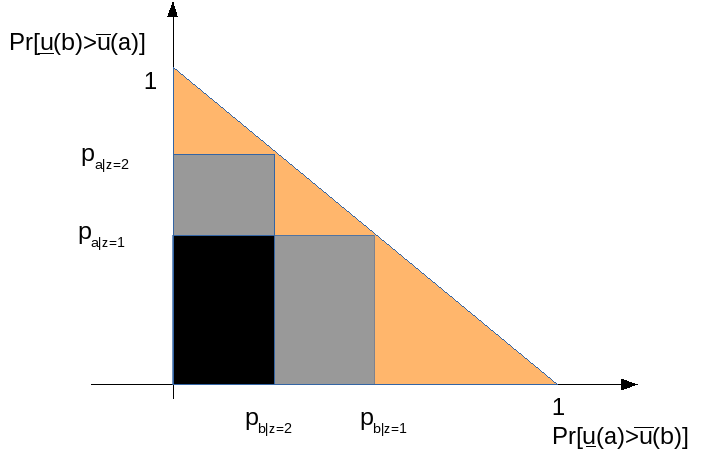
\includegraphics[scale=0.6]{idregion3.png}
    \caption{ID region with an Instrumental Variable}
    \label{fig:IDinstrumental}
\end{figure}

\subsubsection{Imperfect Instruments}

In this section we relax the strong assumption that $\left(
V_{L},V_{U}\right) $ is independent of $Z$. \ \cite{NevoRosen} introduced
the notion of imperfect instrumental variables in a linear regression model
with endogeneous regressors. An imperfect instrumental variable is a
situation where a variable $Z$ is correlated with the error term of the
regression but to a much lesser degree than its correlation with the
endogeneous regressor. \cite{NevoRosen} show that under some conditions this
situation lends itself to partial identification of the regression
parameters. We adjust this notion of imperfect instrumental variables to our
model of choice with vagueness. We define the following quantities.%
\begin{eqnarray*}
\delta _{L} &=&\sup_{z\in \mathcal{Z}}\left\vert \Pr \left(
V_{L}<0|Z=z\right) -\Pr \left( V_{L}<0\right) \right\vert \\
\delta _{U} &=&\sup_{z\in \mathcal{Z}}\left\vert \Pr \left(
V_{U}<0|Z=z\right) -\Pr \left( V_{U}<0\right) \right\vert
\end{eqnarray*}%
and%
\begin{equation*}
\Delta _{0}=\sup_{z\in \mathcal{Z}}p_{0|z}-\inf_{z\in \mathcal{Z}}p_{0|z}.
\end{equation*}

\begin{theorem}
Suppose $\Delta _{0}>\delta _{L}+\delta _{U}$, then $\Pr \left(
V_{U}<0\right) $ is bounded away from $\Pr \left( V_{L}<0\right) $ by a
strictly positive quantity.
\end{theorem}

\begin{proof}
For all $z\in Z$, 
\begin{equation*}
\Pr (V_{U}<0)-\delta _{U}\leq \Pr \left( V_{U}<0|Z=z\right) \leq p_{0|z}
\end{equation*}%
and thus,%
\begin{equation*}
\Pr (V_{U}<0)\leq p_{0|z}+\delta _{U}.
\end{equation*}%
As a result we can say that%
\begin{equation*}
\Pr \left( V_{U}<0\right) \leq \inf_{z\in \mathcal{Z}}p_{0|z}+\delta _{U}.
\end{equation*}%
Similarly, since 
\begin{equation*}
p_{0|z}\leq \Pr \left( V_{L}<0|Z=z\right) \leq \Pr (V_{L}<0)+\delta _{L}.
\end{equation*}%
Using the same steps as above we get that%
\begin{equation*}
\sup_{z\in \mathcal{Z}}p_{0|z}-\delta _{L}\leq \Pr \left( V_{L}<0\right) .
\end{equation*}%
It is now clear that 
\begin{equation*}
\Pr (V_{U}<0)-\Pr \left( V_{L}<0\right) >\Delta _{0}-\delta _{L}-\delta
_{U}>0.
\end{equation*}
\end{proof}

\subsection{Minmax regret}

The observed choice, $y$, is a selection from the random set $Y$. We could
establish only very general bounds on the distribution of $\left(
V_{L},V_{U}\right) $ because we made no assumptions on the selection $y$ in
case in which the consumer cannot compare alternatives. So far, we have been
silent about the way the decision maker makes her choice when $Y\left(
\omega \right) =\left\{ 0,1\right\} $. This approach resulted in partial
identification of the parameters of interest as described above. Next, we
focus on the idea of minimizing maximal regret as a way to break the
consumer's indecision.

Suppose that $\left( V_{L},V_{U}\right) \sim F$ for some joint distribution $%
F$ (it can be a parametric distribution as before). If $V_{U}<0$, the
decision maker chooses choice $0.$ Similarly if $V_{L}>0$, the decision
maker chooses choice $1$. The interesting case occur when $V_{L}<0<V_{U}$.
Both choices in this case may be rational. To break the tie the decision
maker can use the minimax regret rule. In other words, we assume that $y_{i}$
is such that $i$ minimizes the maximum regret she can have when the true
value of choice $1$ is realized. If $i$ chooses $1$, the maximal regret is $%
\left\vert V_{L}\right\vert $ and if $i$ chooses $0$, the maximal regret is $%
V_{U}$. Therefore, $i$ chooses $1$ if $V_{U}\geq \left\vert V_{L}\right\vert 
$ and chooses $0$ otherwise. This is summarized in the following equation.
For each $i$,%
\begin{equation}
y=\left\{ 
\begin{array}{c}
1 \\ 
0%
\end{array}%
\ 
\begin{array}{c}
if\ V_{L}>0\ or\ (V_{L}<0<V_{U}\ and\ V_{U}>|V_{L}|) \\ 
if\ V_{U}<0\ or\ (V_{L}<0<V_{U}\ and\ V_{U}>|V_{L}|)%
\end{array}%
\right. .  \label{minimaxrule}
\end{equation}%
In other words, the minimax regret rule picks one selection from the random
set $Y$. Therefore, $p_{0}=\Pr \left( V_{U}<0\ or\ (V_{L}<0<V_{U}\ and\
V_{U}>|V_{L}|)\right) $. Figure \ref{choiceruleregret} describes the choice
rule in (\ref{minimaxrule}). As one can see, the region where choice was
indeterminate, the ortant where $V_{U}$ is positive and $V_{L}$ is negative,
is now allocated to each alternative so that points above the 45 degree line
mean alternative $1$ is chosen and point below it mean alternative $0$ is
chosen. Adding a parametric assumption on the joint distribution of $\left(
V_{L},V_{U}\right) $ will allow us to point identify the finite parameter of
that distribution. Specifically if we assume that $V_{L}=\bar{V}%
_{L}+\varepsilon $ and $V_{U}=\bar{V}_{U}+\varepsilon $ and $\varepsilon
\sim F_{\varepsilon }$ for a known distribution $F_{\varepsilon }$, then we
can identify the pair $\left( \bar{V}_{L},\bar{V}_{U}\right) $.


\section{Discrete Choice With Knightian Uncertainty}

Next, we discuss how this framework can be extended to allow for ambiguity
and Knightian uncertainty as described in \cite{Bewley86}.\footnote{%
Bewley's original paper has been published recently as \cite{Bewley02}.}
That paper shows that a strict preference relation that is not necessarily
complete, but satisfies all other axioms of the standard Anscombe-Aumann
framework, can be represented by a family of expected utility functions
generated by a unique utility index and a set of probability distributions.%
\footnote{%
Incompleteness in decision making in a Von-Neumann and Morgenstern
environment was first studied by \cite{Aumann62}, which obtains a
representation in which the probability is unique but there are multiple
utility functions.} Lack of completeness is thus reflected in multiplicity
of beliefs: the unique subjective probability distribution of the standard
expected utility framework is replaced by a set of probability
distributions, and when the preference relation is complete this set becomes
a singleton.

We let $S$ denote the state space and, with abuse of notation, also the
cardinality of that space. There are $J$ possible choices, and the utility
of each choice depends on the state that is realized. Therefore, for each
choice $j\in J$ we specify the utility that choice yields in each state.
Formally, the utility of an individual for choice $j$ in state $s$ is
denoted as $u\left( j,s\right) $. Let $\Delta (S)$ be the set of all
probability distributions over $S$. If $\pi \in \Delta (S)$, the expected
utility of individual $i$ according to that probability is given by 
\begin{equation*}
E_{\pi }\left[ u\left( j\right) \right] \equiv \sum_{s\in S}\pi \left(
s\right) u\left( j,s\right)
\end{equation*}%
Bewley's theory provides axioms on decision maker $i$'s preferences $\succ $%
; under these axioms there exists a closed and convex set $\Pi $ of
probability distributions on $S$ with the property that 
\begin{equation*}
j\succ k\qquad \text{if and only if}\qquad E_{\pi }\left[ u\left( j\right) %
\right] >E_{\pi }\left[ u\left( k\right) \right] \text{ for all }\pi \in \Pi
\end{equation*}%
If the inequality changes sign for different probability distributions the
two alternatives are not comparable. This is not a special case of the
interval order we studied in the previous section. Although all the possible
values of $E_{\pi }\left[ u_{i}\left( j\right) \right] $ describe an
interval as before, comparisons are made one probability distribution at the
time and not by looking at the extremes of that interval; two alternatives
could be ranked even if the corresponding intervals overlap. Despite this
difference, the results of the previous section can be applied here by
taking advantage of some simple algebra.

The expression above can be rewritten in terms of the expected value of the
utility difference between the two alternatives as:%
\begin{equation*}
j\succ k\qquad \text{if and only if}\qquad E_{\pi }\left[ u\left( j\right)
-u\left( k\right) \right] >0\text{ for all }\pi \in \Pi
\end{equation*}%
and therefore one obtains%
\begin{equation*}
j\succ k\qquad \text{if and only if}\qquad E_{\pi ^{min}}\left[ u\left(
j\right) -u\left( k\right) \right] >0
\end{equation*}%
and 
\begin{equation*}
k\succ j\qquad \text{if and only if}\qquad E_{\pi ^{max}}\left[ u\left(
j\right) -u\left( k\right) \right] <0,
\end{equation*}%
where we defined $\pi ^{min}\in \arg \min_{\pi \in \Pi }E_{\pi }\left[
u\left( j\right) -u\left( k\right) \right] $ and $\pi ^{max}\in \arg
\max_{\pi \in \Pi }E_{\pi }\left[ u\left( j\right) -u\left( k\right) \right] 
$. This last two inequalities can now be used

Suppose the choice set $\mathcal{C}$ contains only alternatives $j$ and $k$.
Then, the decision maker's choices can be described by the following set%
\begin{equation*}
Y=\left\{ 
\begin{array}{c}
\{j\} \\ 
\{j,k\} \\ 
\{k\}%
\end{array}%
\ 
\begin{array}{c}
if\ E_{\pi ^{min}}\left[ u\left( j\right) -u\left( k\right) \right] >0 \\ 
0\in \left[ E_{\pi ^{min}}\left[ u\left( j\right) -u\left( k\right) \right]
,E_{\pi ^{max}}\left[ u\left( j\right) -u\left( k\right) \right] \right] \\ 
if\ E_{\pi ^{max}}\left[ u\left( j\right) -u\left( k\right) \right] <0%
\end{array}%
\right. .
\end{equation*}%
At this point, the same logic of the previous set can be applied to try and
identify properties of the probability distribution of $E_{\pi ^{min}}\left[
u\left( j\right) -u\left( k\right) \right] $ and $E_{\pi ^{max}}\left[
u\left( j\right) -u\left( k\right) \right] $. Before illustrating this,
however, note that individuals' choices will not reveal details about the
distribution of $\Pi $ and $u\left( \cdot \right) $ (the preference
parameters) beyond what one may learn from the two extreme expectations.

From now on, think of $E_{\pi ^{min}}\left[ u\left( j\right) -u\left(
k\right) \right] $ and $E_{\pi ^{max}}\left[ u\left( j\right) -u\left(
k\right) \right] $ as two random variables which obviously satisfy $\Pr
\left( E_{\pi ^{min}}\left[ u\left( j\right) -u\left( k\right) \right] \leq
E_{\pi ^{max}}\left[ u\left( j\right) -u\left( k\right) \right] \right) =1$.
In other words, while consumers may differ in either their utility function
for each alternative or in the probability they assign to each state of the
world, the only heterogeneity data can be informative about is the one of
these extreme expected values. As we observe individuals' choice that follow
the rule illustrated by the set $Y$, we use these observations to learn
about some features of the distribution of these random variables. By
applying Artstein's inequality here, we observe the following. When $%
K=\left\{ j\right\} $, we have 
\begin{equation*}
C_{Y}\left( \{j\}\right) =\Pr \left( Y\subset \{j\}\right) =\Pr \left(
E_{\pi ^{min}}\left[ u\left( j\right) -u\left( k\right) \right] >0\right) ,
\end{equation*}%
while when $K=\left\{ k\right\} $ we obtain 
\begin{equation*}
C_{Y}\left( \left\{ k\right\} \right) =\Pr \left( Y\subset \{k\}\right) =\Pr
\left( E_{\pi ^{max}}\left[ u\left( j\right) -u\left( k\right) \right]
<0\right) .
\end{equation*}%
Therefore, from Artstein inequality we conclude that%
\begin{equation*}
\Pr (y=j)\geq \Pr \left( E_{\pi ^{min}}\left[ u\left( j\right) -u\left(
k\right) \right] >0\right)
\end{equation*}%
and 
\begin{equation*}
\Pr \left( y=k\right) \geq \Pr \left( E_{\pi ^{max}}\left[ u\left( j\right)
-u\left( k\right) \right] <0\right)
\end{equation*}%
Using the fact that $\Pr \left( y=j\right) =1-\Pr (y=k)$, we can conclude
that 
\begin{equation*}
\Pr \left( E_{\pi ^{min}}\left[ u\left( j\right) -u\left( k\right) \right]
>0\right) \leq \Pr (y=j)\leq \Pr \left( E_{\pi ^{max}}\left[ u\left(
j\right) -u\left( k\right) \right] >0\right) .
\end{equation*}

As before, if the data identifies the values of $p_{k}$ and $p_{j}$ as the
probability that a randomly chosen individual will choose $k$ and $j$
respectively, the inequalities above imply that 
\begin{equation*}
\Pr \left( E_{\pi ^{min}}\left[ u\left( j\right) -u\left( k\right) \right]
>0\right) \leq p_{j}\leq \Pr \left( E_{\pi ^{max}}\left[ u\left( j\right)
-u\left( k\right) \right] <0\right) .
\end{equation*}%
Thus, knowledge about the probability that a randomly chosen individual will
choose $j$ implies restrictions on the marginal distributions of $E_{\pi
^{min}}\left[ u\left( j\right) -u\left( k\right) \right] $ and $E_{\pi
^{max}}\left[ u\left( j\right) -u\left( k\right) \right] $. In particular,
the lowest expected utility difference between $j$ and $k$ cannot be smaller
that the probability of choosing $j$, and the largest expected utility
difference between $j$ and $k$ cannot be larger that the probability of
choosing $j$.\ So, the inequality above says that data can impose
restrictions on preference parameters even when the underlying preferences
are not complete.

\subsection{Epsilon-contamination model}

We now specialize the model of decision making under uncertainty so that we
can learn more details about preferences from the partially identified
region for the probability distribution of the highest and lowest
expectations. In particular, we assume that $S$ has only two elements
(denoted $H$ and $L$) and that $\Pi =\left\{ (1-\varepsilon )\hat{\pi}%
+\varepsilon \pi :\pi \in \Delta ^{2}\right\} $ where $\Delta ^{2}$ is the
two dimensional simplex and $\varepsilon $ is a random variable that takes
values in the interval $\left[ 0,1\right] $. This is known as the $%
\varepsilon $-contamination model as the set $\Pi $ is constructed by
\textquotedblleft mixing\textquotedblright\ a reference distribution with
arbitrary distributions in the simplex. One can think of it as building a
probabilistic neighborhood of size epsilon around the reference measure. The
size of $\varepsilon $ is then a measure of the amount of ambiguity.

Consumers face two choices $\left\{ j,k\right\} $, and for simplicity we
assume that $u\left( j\right) =0$ in all states of the world.\footnote{%
By setting the utility of one option constant, we collapse reduce the model
of this section to the one of the previous section, in that the upper and
lower bounds on the expected utility of the uncertain options determine
behavior.} For option $k$, however, we assume the utility of each consumer
can be either $u_{L}$ or $u_{H}$, with $u_{L}<0<u_{H}$, depending on the
state of the world. The reference probability distribution is $\hat{\pi}%
=\left( \hat{\pi}_{L},\hat{\pi}_{H}\right) $. By construction, the
probabilities assigned to state $L$ satisfy%
\begin{equation*}
\left( 1-\varepsilon \right) \hat{\pi}_{L}\leq \pi _{L}\leq \left(
1-\varepsilon \right) \hat{\pi}_{L}+\varepsilon
\end{equation*}%
The bounds on the probability assigned to state $L$ induce bounds on the
expected utility from choosing option $k$; in particular,%
\begin{eqnarray*}
E_{\hat{\pi}}\left[ u\left( k\right) \right] &=&\hat{\pi}_{L}u_{L}+\hat{\pi}%
_{H}u_{H}+\left( \pi _{L}-\hat{\pi}_{L}\right) \varepsilon u_{L}+\left( \pi
_{H}-\hat{\pi}_{H}\right) \varepsilon u_{H} \\
&=&\bar{U}+\varepsilon \left[ \left( \pi _{L}-\hat{\pi}_{L}\right)
u_{L}+\left( \pi _{H}-\hat{\pi}_{H}\right) u_{H}\right] \\
&=&\bar{U}+\varepsilon \left[ \pi _{L}u_{L}+\pi _{H}u_{H}-\bar{U}\right]
\end{eqnarray*}%
where we use $\bar{U}$ to denote the expected utility of alternative $k$
according to the reference measure ($\bar{U}=\hat{\pi}_{L}u_{L}+\hat{\pi}%
_{H}u_{H}$). Therefore, since $u_{L}<0<u_{H}$, the highest and lowest
expected utility are given by%
\begin{equation*}
\bar{U}+\varepsilon \left( u_{H}-\bar{U}\right) \quad \text{and}\quad \bar{U}%
+\varepsilon \left( u_{L}-\bar{U}\right)
\end{equation*}%
respectively.

We can now use the inequalities implied by Artstein's inequality (here we
use $\bar{U}-\varepsilon \left( \bar{U}-u_{L}\right) $ instead of $V_{L}$,
and $\bar{U}+\varepsilon \left( u_{H}-\bar{U}\right) $ instead of $V_{U}$).
to derive that 
\begin{equation*}
\Pr \left( \bar{U}-\varepsilon \left( \bar{U}-u_{L}\right) <0\right) \geq
p_{0}\geq \Pr \left( \bar{U}+\varepsilon \left( u_{H}-\bar{U}\right)
<0\right) .
\end{equation*}%
These inequalities imply inequalities on the CDF\ of $\varepsilon $. With
some algebra we can show that

\begin{equation}
\Pr \left( \bar{U}-\varepsilon \left( \bar{U}-u_{L}\right) <0\right) =\Pr
\left( \varepsilon >\frac{\bar{U}}{\left( \bar{U}-u_{L}\right) }\right)
\label{Lconstraint}
\end{equation}%
and 
\begin{equation}
\Pr \left( \bar{U}+\varepsilon \left( u_{H}-\bar{U}\right) <0\right) =\Pr
\left( \varepsilon <-\frac{\bar{U}}{\left( u_{H}-\bar{U}\right) }\right) .
\label{Uconstraint}
\end{equation}%
By definition, we have that $u_{L}\leq \bar{U}\leq u_{H}$. If $\bar{U}>0$,
then the constraint (\ref{Uconstraint}) is non binding since $\Pr \left( 
\bar{U}+\varepsilon \left( u_{H}-\bar{U}\right) <0\right) $ is trivially
zero. On the other hand if $\bar{U}<0$, then the constraint in (\ref%
{Lconstraint}) is non binding since $\Pr \left( \bar{U}-\varepsilon \left( 
\bar{U}-u_{L}\right) <0\right) $ is trivially zero.

Let $\theta =\left( \hat{\pi},u_{L},u_{H},F_{\varepsilon }\right) \in \Theta
=\Delta ^{2}\times \mathbb{R}_{-} \times \mathbb{R}_{+}\times \Gamma $ be the parameter space where $\Gamma $ is the set of all
random variables on $\left[ 0,1\right] $. Using the definition of the
identification region in (\ref{ID1}) we can write the identification region
of the parameter $\theta $. It is easy to see that $\Theta $ is too high
dimensional and the identification region $\Theta _{I}$ in (\ref{ID1}) is
hard to characterize. At this point it is useful to fix some of the
dimensions and see what information can be drawn on the remaining
dimensions. We explore some of these options below by assuming that the
utility of option $k$ in each state as well as the probability distribution $%
\hat{\pi}$ are the same for all consumer. In this case, the only source of
heterogeneity is given by differences in the perception of ambiguity.

\textbf{Example}. Suppose $\hat{\pi},u_{L}$ and $u_{H}$ are fixed and $%
\varepsilon $ is distributed $B\left( \alpha ,\beta \right) $ for unknown $%
\alpha $ and $\beta $. The identification region is all the pairs of $\alpha 
$ and $\beta $ such that (\ref{Lconstraint}) and (\ref{Uconstraint}) are
satisfied. Figure (\ref{BetaID}) shows the possible pairs of $(\alpha ,\beta
)$ for $\hat{\pi}=\left( 0.6,0.4\right) $, $u_{L}=-2,$ $u_{H}=1$ and $%
p_{0}=0.37$.

Moreover, we can compute the identification rage for the average and
variance\ of $\varepsilon $. In the example above, the Beta distributions
admitted into the identification region have an expectation ranging from $%
0.55$ to $1$ and a variance of at most $0.22$. These numbers tell us about
the degree of ambiguity faced by the agents as suggested by the data.
Intuitively, the degree of ambiguity is high enough to offset the negative
expected value of alternative $k$.


\section{Voting and Abstaining}\label{Voting}

Until this point we assumed that agents have to make a choice from the set
of alternatives $\mathcal{A}$. The important part of this assumption is that
a utility is assigned to each of the elements in the set $\mathcal{A}$,
potentially an interval. It is possible that $\mathcal{A}$ contains a 'no
action' alternative (e.g. do not buy any car) but this alternative gives a
certain utility to the DM which is often normalized to zero. There are
situations where the DM can abstain from making any choice. The most
prominent example is voting. When a DM (voter) comes to the polling place
she can chose to abstain from voting on some or all of the races on the
ballot. The utility associated with this choice is undefined. Denote the
extended alternatives set as,%
\begin{equation*}
\mathcal{\bar{A}}=\mathcal{A}\cup \left\{ \emptyset \right\} .
\end{equation*}%
In the case of voting, by abstaining the DM delegates the decision to other
DMs.

\subsection{Voting in Ohio}

We apply the theory described above to voting in Ohio. The voting in Ohio
presents a neat IV example. It is known that the order of the candidates on
the ballot affects the chances of candidates to be elected. As a result ordering the candidates in alphabetical order may bias the
results in favor of candidates with certain family names.

To be completed

\section{Conclusions}\label{conclustions}
TBA

%%%%%%%%%%%%%%%%%%%%%%%%%%%%
%%% Technical Appendices %%%
%%%%%%%%%%%%%%%%%%%%%%%%%%%%
\newpage 
\appendix
%%%%% Appendix A %%%%%
\appendixpage
\section{Technical Results For Section \ref{nonpar} }\label{nonparAppendix}
To demonstrate the effect of Artstein's Lemma we prove the following two claims related to the sharpness of the identification set $\mathcal{P}^I$ defined in equation (\ref{idRegion}) in Section \ref{nonpar}. First we show that $\mathcal{P}^I$ is a strict subset of $\mathcal{P}$ under mild conditions. We then show that all the inequality implied by Artstein's Lemma are potentially binding. 
\begin{claim}
$\mathcal{P}^{I}$ is a strict subset of $\mathcal{P}$ if $\exists a \in A$ such that $1 >\Pr (y=a) >0$.
\end{claim}

\begin{proof}
There is $a^{ \prime } \neq a$ such that $\Pr (y =a^{ \prime }) >0$.
Therefore, $\Pr (\text{\b{u}}(a) >\bar{u} (a^{ \prime })) <1$. This is a restriction on the joint distribution of $\{\text{\b{u}} (a) ,\bar{u} (a)\}_{a \in A}$ that is not included in the definition of $\mathcal{P}$. Therefore, $\mathcal{P}^{I}$ is a strict subset of $\mathcal{P}$.
\end{proof}

We now want to demonstrate that the conditions in Artstein's Lemma essential in the sense that using less restrictions yields a strictly larger set than the identification region. Let 
\begin{equation*}
\mathcal{P}^{1}=\{P\in \mathcal{P} :C_{M}(\{a\})\leq \Pr (y=a) \text{ } \forall a\in A\}
\end{equation*}%
be the set of joint distributions that satisfy Artstein's Lemma only for subsets of $A \subset \mathcal{A}$ of cardinality $1$.

\begin{claim}
If $\vert \mathcal{A}\vert >2$, $\mathcal{P}^{I} \subsetneqq \mathcal{P}^1$.
\end{claim}

\begin{proof}
Since $\vert \mathcal{A}\vert >2$ and $\vert A \vert =1$, there are two alternatives $a ,a^{ \prime } \in \mathcal{A}$ such that $a \neq a^{ \prime }$ and $\{a ,a^{ \prime }\} \neq A$. By Artstein's Lemma $C_{M} (\{a\}) \leq \Pr (y =a)$, $C_{M} (a^{ \prime }) \leq \Pr (y =a^{ \prime })$ and $C_{M} (\{a ,a^{ \prime }\}) \leq \Pr (y \in \{a ,a^{ \prime }\})$. The first two inequalities yield $C_{M} (\{a\}) +C_{M} (\{a^{ \prime }\}) \leq \Pr (y =a) +\Pr (y =a^{ \prime }) =\Pr (y \in \{a ,a^{ \prime }\})$ where the last equality is implied by $a \neq a^{ \prime }$. This inequality is included in the definition of $P^{1}$. Since $C_{M} (\{a\}) +C_{M} (\{a^{ \prime }\}) \leq C_{M} (\{a ,a^{ \prime }\})$, the inequality $C_{M} (\{a ,a^{ \prime }\}) \leq \Pr (y \in \{a ,a^{ \prime }\})$ may impose an additional restriction on the distribution of $y$ and therefore on the joint distribution of $\{ \text{\b{u}} (a) ,\bar{u} (a)\}_{a \in A}$.
\end{proof}

%%%%% Appendix B %%%%%
\section{Incomplete Probit Example}

Consider the following binary choice model. Let $\mathcal{A}=\left\{
0,1\right\} $ be the alternatives set. Normalize the utility from choice $%
u_{i}\left( 0\right) =0$ for all $i$. The utility from choice $1$ is vague.
we assume that $u_{i}\left( 1\right) \in \left[ \beta _{i},\beta _{i}+\delta
_{i}\right] $ where $\delta _{i}>0$ and the joint distribution of $\left(
\beta ,\delta \right) $ is unknown. From Artstein's inequalities we know that%
\begin{equation*}
\Pr \left( \beta +\delta <0\right) \leq p_{0}\leq \Pr \left( \beta <0\right)
.
\end{equation*}%
These two inequalities impose a certain restrictions on the joint
distribution of $\left( \beta ,\delta \right) $ but these restrictions are
limited.

\subsection{One dimensional heterogeneity}

Suppose now that $\beta _{i}=\beta -\varepsilon _{i}$ where $\varepsilon
_{i}\sim F_{\varepsilon }$ for a known distribution $F_{\varepsilon }$ (e.g.
a logistic or standard normal distribution). $\delta $ is assumed to be
constant across all decision maker. In other words, there is only one source
of heterogeneity. This implies that the following is an equivalent model.
Set $u_{i}\left( 0\right) =\varepsilon _{i}$ with $\varepsilon _{i}\sim
F_{\varepsilon }$ and $u_{i}\left( 1\right) =\beta +\delta $ constant for
all $i$.

Under these assumptions, $\Pr \left( \beta <0\right) =1-F_{\varepsilon
}\left( \beta \right) $ and $\Pr \left( \beta +\delta <0\right)
=1-F_{\varepsilon }\left( \beta +\delta \right) $. Since $p_{0}=1-p_{1}$, we
can write 
\begin{equation*}
F_{\varepsilon }\left( \beta +\delta \right) \leq p_{1}\leq F_{\varepsilon
}\left( \beta \right) ,
\end{equation*}%
or%
\begin{equation*}
\beta \leq F_{\varepsilon }^{-1}\left( p_{1}\right) \leq \beta +\delta .
\end{equation*}%
The identification region is, therefore, 
\begin{equation*}
\Theta ^{I}=\left\{ \left( \beta ,\delta \right) \in \mathbb{R} \times \mathbb{R}_{+}:\beta \leq F_{\varepsilon }^{-1}\left( p_{1}\right) \leq \beta +\delta
\right\} .
\end{equation*}%
As before, suppose there is an additional variable $z$ independent of $%
\left( \beta ,\delta \right) $ with support $\mathcal{Z}$. In that case,%
\begin{equation*}
\Theta ^{I}=\left\{ \left( \beta ,\delta \right) \in \mathbb{R} \times \mathbb{R}_{+}:\beta \leq \inf_{z\in \mathcal{Z}}F_{\varepsilon }^{-1}\left(
p_{0}|z\right) \ and\ \sup_{z\in \mathcal{Z}}F_{\varepsilon }^{-1}\left(
p_{0}|z\right) \leq \beta +\delta \right\} .
\end{equation*}

\begin{figure}[h!]
    \centering
    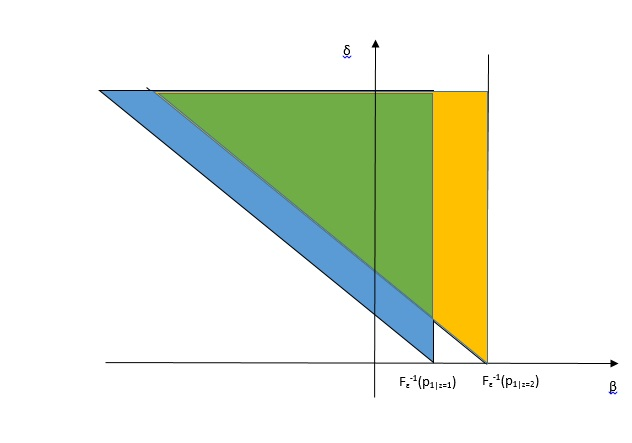
\includegraphics[scale=0.6]{oneDimHetero.jpg}
    \caption{One Dimensional Heterogeneity}
    \label{fig:oneDimHetero}
\end{figure}

\subsection{Two dimensional heterogeneity}

Here we add an additional source of heterogeneity - the amount of vagueness.
Let $\sigma _{i}=\sigma -\eta _{i}$ for each $i$. Using the same logic as
before, we get%
\begin{equation*}
\Pr (\varepsilon _{i}\leq \beta )\leq p_{1}\leq \Pr \left( \varepsilon
_{i}+\eta _{i}\leq \beta +\delta \right) .
\end{equation*}%
These inequalities translate to 
\begin{eqnarray*}
\beta &\leq &F_{\varepsilon }^{-1}\left( p_{1}\right) \\
F_{\varepsilon +\eta }^{-1}\left( p_{1}\right) &\leq &\beta +\delta .
\end{eqnarray*}%
The identification set is defined accordingly. Suppose $\beta_{i}\sim
N(\beta ,\sigma_{\beta }^{2})$ and $\delta_{i}\sim Exp\left( \frac{1}{\delta }\right)$ independent of $\beta_{i}$. Collecting the parameters we have $\theta =\left( \beta ,\sigma _{\beta }^{2},\delta \right)$. Note that $\beta_{i}+\delta_{i}$ distribution is called Exponentially Modified Gaussian (EMG)\ distribution.\footnote{%
Let $\lambda =\frac{1}{\delta }$, then the CDF of an EMG distribution is
given by $EMG(z;\beta ,\sigma _{\beta }^{2},\lambda )=\frac{1}{2}\left[
1-q_{1}\cdot q_{2}+q_{3}\right] $ where $q_{1}=\exp \left[ \lambda \left( 
\frac{\lambda \sigma _{\beta }^{2}}{2}+\mu +z\right) \right] $, $q_{2}=1-\operatorname{erfc}\left( \frac{\sigma _{\beta }}{\sqrt{2}}\left( \lambda +\frac{%
\beta -z}{\sigma _{\beta }^{2}}\right) \right) $, $q_{3}=\operatorname{erfc}\left( 
\frac{1}{\sqrt{2}\sigma _{\beta }}\left( z-\mu \right) \right) $ and $\operatorname{erfc}\left( t\right) =\frac{2}{\sqrt{\pi }}\int_{0}^{t}\exp \left(
-x^{2}\right) dx$ is the error function.}
\maketitle

\break
\bibliography{ambiguity}

\end{document}
